\section{Lezione 16}%
\label{sub:Lezione 16}
\subsection{Trasformazioni canoniche}%
\label{sub:Trasformazioni canoniche}
\begin{redbox}{}
    Una trasformazione canonica è un cambio di variabili generalizzate tale che:
    \[
        H(p_i, q_i) = H'(P_i(p_i,q_i), Q_i(p_i, q_i) ) 
    .\] 
    Le nuove variabili devono rispettare le regole di commutazione canoniche:
    \[
	\dot{Q}_i = - \left[ Q_i,H\right] \qquad \dot{P}_i = \left[P_i, H\right]
    .\] 
\end{redbox}
\noindent
Spesso nello studio dei sistemi Hamiltoninani è necessario trovare delle trasformazioni che permettano di integrare H. \\
Integrare l'Hamiltoniana significa trovare le $P_i, Q_i$  tali che:
\[
    H(p_i, q_i) \to H'(P_i) 
.\] 
Quindi per le equazioni di Hamilton-Jacoby anche:
\[\begin{aligned}
    & \dot{P}_i = - \frac{\partial H'}{\partial Q_i} =0\\
    & \dot{Q}_i = \frac{\partial H'}{\partial P_i} = f_i(P_i) 
.\end{aligned}\]
Questo ci permette di trovare una equazione del moto come:
\[
    \dot{Q}_i = f_i(P_i) t + Q_i(0) 
.\] 
Per ottenere una trasformazione canonica è necessario passare dalle \textbf{Funzioni generatrici}.\\
Per trovare queste funzioni partiamo dalla considerazione che $H$ conserva il volume nello spazio delle fasi, quindi anche $H'$ deve conservare tale volume:
\[
    \int\int dpdq = \int\int dPdQ
.\] 
Quindi possiamo sfruttare il teorema di stokes:
\[
    \oint pdq = \oint  QdP
.\] 
\begin{equation}
    \oint  \left[pdq - QdP\right] = 0 
    \label{eq:16_stokes}
\end{equation}
Grazie a questo integrale possiamo riscrivere tutto in funzione di $q$ e $P$.\\
La quantità nell'integrale di linea \ref{eq:16_stokes} è il differenziale di una qualche funzione $F_2$:
\[
    \oint dF_2(q,P) = \oint \frac{\partial F_2}{\partial q} dq + \frac{\partial F_2}{\partial P} dP = 0 
.\] 
Quindi:
\[\begin{aligned}
    &p = \partial_{q}F_2(q,P) \\
    &Q = - \partial_{P}F_2(q,P) 
.\end{aligned}\]
Notiamo che aver scritto tutto in funzione della coppia $(q,P)$ è una scelta (che conduce al funzionale chiamato storicamente $F_2$), si potevano effettuare altre scelte ottenendo lo stesso formalismo con funzionali dipendenti dalle coppie scelte.\\
Quello che interessa a noi è trovare la trasformazione furba che ci permetta di integrare l'Hamiltoniana.
\subsection{Ricerca della trasformazione che integra $H$}%
\label{sub:Ricerca della trasformazione per integrare H}
Supponiamo che la trasformazione ideale sia $S(\vect{q}, \vect{\alpha})$, con $\vect{\alpha}$ nuovi momenti conservati (quelli che prima erano $P$). Analogamente definiamo le $Q$ ideali per la trasformazione come $\beta$.\\
Esplicitiamo le equazioni del cambio di vaiabili in questo caso:
\[
    p_i = \frac{\partial S}{\partial q_i} \qquad \beta_i = - \frac{\partial S}{\partial \alpha_i} 
.\] 
Esplicitando queste trasformazioni nella dipendenza da $p_i$ di $H$ si ottiene:
\[
    H(\vect{q}, \frac{\partial S}{\partial \vect{q}}) = H'(\vect{\alpha}) 
.\] 
Quindi questa equazione ci permette di esprimere delle Equazioni di HJ, tramite tali equazioni possiamo invertire e trovare $\partial_{q}S$, infine di integra per trovare la $S$ ideale.\\
In generale risolvere il problema è molto complicato, per semplificare il calcolo dobbiamo considerare il fatto che gli $\vect{\alpha}$ sono delle costanti del moto
\footnote{Per definizione della trasformazione che cerchiamo si ha che $\dot{\alpha}_i = -\partial_{\beta}H' = 0$ }
. Tenendo conto di questo il differenziale della derivata di $S$ ($dS'$) si esprime come:
\[
    dS' = \sum_{}^{} \frac{\partial S}{\partial q_i} dq_i = \sum_{}^{} P_idq_i
.\] 
ed integrando si ha direttamente:
\[
    S = \int_{q_0}^{q_t} \sum_{i}^{} P_idq_i 
.\] 
\begin{exmp}[Hamiltoniana 1D]
    Prendiamo una trasformazione nello spazio unidimensionale tale che:
    \[
	H(q,\partial_{q}S) = H'(\alpha) = \alpha
    .\] 
    Le coordinate dipendenti possono essere espresse tramite la trasformazione (ignota) come:
    \[\begin{aligned}
	& p = \partial_{q}S(q, \alpha) \\
	& \beta  = \partial_{\alpha}S(q, \alpha) 
    .\end{aligned}\]
    Le equazioni HJ sono:
    \[\begin{aligned}
	&\dot{\alpha}= - \partial_{\beta} H' = 0\\
	&\dot{\beta} = \partial_{\alpha}H' = 1
    .\end{aligned}\]
    Possiamo integrare quindi per $\beta$ (imponiamo che $\beta (t=0) =0$):
    \[
        \beta  = t-t_0
    .\] 
    Quindi abbiamo che:
    \[\begin{aligned}
	t-t_0 =& \int dt \dot{\beta} 
	       = \int_{q_0}^{q_t} d\beta (q) \\
	       & = \int_{q_0}^{q_t} \partial_{q}\beta dq 
	       = \int  \partial_{q}\partial_{\alpha}S dq = \\
	       & = \int\partial_{\alpha }\partial_{q}Sdq
	       = \int_{q_0}^{q_t} \partial_{\alpha}P(q, \alpha) dq 
    .\end{aligned}\]
    In definitiva possiamo scrivere il $t-t_0$ in funzione di quell'ultimo integrale:
    \[
        t-t_0 = \int_{q_0}^{q_t} \partial_{\alpha}P(q, \alpha) dq 
    .\] 
\end{exmp}
\noindent
\begin{exmp}[Moto in potenziale a energia fissa]
    Prendiamo l'Hamiltoniana unidimensionale con un potenziale:
    \[
	H = \frac{p^2}{2} + V(q) = \alpha
    .\] 
    In questo caso il nuovo momento della trasformazione è l'energia del sistema.\\
    Esplicitiamo $P(q,\alpha)$ in funzione delle variabili selezionate:
    \[
	P(q,\alpha) = \sqrt{2(\alpha-V(q))} 
    .\] 
    Quindi otteniamo un tempo $t-t_0$ che rappresenta il periodo del moto:
    \[
	t-t_0 = \int_{q_0}^{q_t} \frac{1}{\sqrt{2(\alpha-V(q))}}dq 
    .\] 
\end{exmp}
\noindent
\begin{exmp}[Moto in campo centrale]
    \[
	H = \frac{p^2_r}{2} + \frac{p_\phi^2}{2r^2} + V(r) 
    .\] 
    In questo caso abbiamo un momento conservato: $p_\phi$, quindi abbiamo una quantità per il moto $\alpha_\phi$ che si conserva. Possiamo scrivere in tal caso:
    \[
	S(\vect{q}, \vect{\alpha}) = \alpha_\phi\phi  + S_1(r, \alpha_1) 
    .\] 
    In questo modo sappiamo che derivando rispetto a $\phi$  si ottiene la quantità conservata.\\
    Riscriviamo l'Hamiltoniana:
    \[
	H' = \frac{1}{2}\left[(\partial_{r}S_1)^2 + \frac{\alpha_\phi^2}{r^2}\right] + V(r) = \alpha_1
    .\] 
    Scriviamo l'equazione per l'incognita: $\partial_{r}S_1$:
    \[
	\partial_{r}S_1 = \sqrt{2\left[\alpha_1 - V(r) \right]- \frac{\alpha_\phi^2}{r^2}} 
    .\] 
    Questa equazione può essere integrata, si ottiene immediatamente che:
    \[
        S = \alpha_\phi\phi  + \int dr \sqrt{2\left[\alpha_1 - V(r) \right]- \frac{\alpha_\phi^2}{r^2}} 
    .\] 
    A questo punto si fanno i passaggi dell'esempio precedente (c'è un cambio di notazione: $-t_0\to \beta_1$), quindi si ha:
    \[
	\beta_1 + t = \frac{\partial S}{\partial \alpha_1} = \int  \frac{dr}{\sqrt{2(\alpha_1-V(r))- \alpha^2_\phi  /r^2}}
    .\] 
    \[
	\beta_2 = \frac{\partial S}{\partial \alpha_\phi} = \int  \frac{d\phi}{\sqrt{2(\alpha_1-V(r))- \alpha^2_\phi  /r^2}} + \phi
    .\] 
    Notiamo che non aver inserito la dipendenza dal tempo per $\beta_2$ è una conseguenza di tutto il meccanismo utilizzato: deriva direttamente dalle equazioni d Hamilton:
    \[
        H' = \alpha_1 \implies  \frac{\partial H'}{\partial \alpha_\phi} = 0 = \dot{\beta_2}
    .\] 
\end{exmp}
\noindent
\subsection{Variabili azione-angolo in una dimensione}%
\label{sub:Variabili azione-angolo}
Partiamo con la seguente:
\begin{redbox}{}
    Per Hamiltoniane limitate in 1D il moto nello spazio delle fasi avviene sempre su traiettorie chiuse.
\end{redbox}
\noindent
Di conseguenza potremmo cercare una variabile angolo $\theta$ che aumenti di $2\pi$ dopo un giro. Definiamo il momento coniugato di questa variabile come $I$
\footnote{Il motivo per il quale storicamente è di interesse proprio questa trasformazione è che venne studiata per valutare la stabilità del sistema solare}.\\
La trasformazione canonica cercata è $S(q, I)$.
\[
    p = \partial_{q}S(q,I) \qquad \theta  = \partial_{I}S(q,I) 
.\] 
Inoltre dobbiamo fare in modo che la trasformazione permetta di integrare l'Hamiltoniana, serve quindi che:
\[
    H(q, \partial_{q}S) = \alpha  = H'(I) 
.\] 
Il fatto che la variabile $\theta$ sia periodica porta con se il vantaggio di poter fare teoria delle perturbazioni, come approfondiremo nella prossima lezione.\\
Procediamo supponendo $\alpha$ costante e fissato. 
\[
    \partial_{q}\theta  = \partial_{q}\partial_{I}S = \partial_{I}\partial_{q}S \ ( = \partial_{I}P(I) ) 
.\] 
Visto che dopo un giro si ha che: $\theta\to \theta +2\pi$.
\[
    2\pi  = \oint _c d\theta  = \frac{\partial }{\partial I} \oint \frac{\partial S}{\partial q} dq = \frac{\partial }{\partial I} \oint p dq 
.\] 
Questo implica un importante teorema:
\begin{redbox}{}
    \[
        \oint pdq = 2\pi I 
    .\] 
    quindi abbiamo una azione (fissata una curva chiusa nello spazio delle fasi):
    \[
        I = \frac{1}{2\pi}\oint_c pdq 
    .\] 
\end{redbox}
\noindent
Operativamente quello che si fa per risolvere è:
\begin{itemize}
    \item Si risolve l'Hamiltoniana nel cambio di variabili:
	\[
	    H(q,\partial_{q}S) = \alpha
	.\] 
    \item Si calcola l'azione $I$ con la formula sopra sulle curve $c$ che hanno $\alpha$ costante.
\end{itemize}
Le equazioni canoniche per le nuove variabili $I,\theta$ sono:
\begin{redbox}{}
\[
    \dot{I}=-\partial_{\theta  }H'(I) = 0 \qquad \dot{\theta} = \partial_{I}H'(I) = \omega (I) 
.\]    
\end{redbox}
\noindent
Visto che la $I$  è costante nel tempo integriamo l'equazione per $\dot{\theta}$  ottenendo:
\[
    \theta (t) = \omega (I) t + \theta_0
.\] 
La cosa importante è che tutta la fisica del problema è inclusa nella dipendenza di $\omega$  dall'azione $I$.
\begin{exmp}[Oscillatore armonico]
    Prendiamo l'equazione per un oscillatore armonico unidimensionale:
    \[
        H = \frac{p^2}{2} + \frac{\omega^2_0 q^2}{2}
    .\] 
    Abbiamo come sempre che
    \[
        p = \frac{\partial S}{\partial q} 
    .\] 
    Quindi l'Hamiltoniana si esprime come:
    \[
        \frac{1}{2}\left(\frac{\partial S}{\partial q} \right)^2 + \frac{1}{2} \omega_0^2q^2 = \alpha
    .\] 
    Passiamo direttamente alla ricerca della azione $I$:
    \[
	I = \frac{1}{2\pi}\oint pdq = \frac{1}{2\pi}\oint _c \sqrt{2(\alpha-\frac{1}{2}\omega_0^2q^2) }dq = \frac{\alpha}{\omega_0}
    .\] 
    Possiamo trovare anche il periodo del moto e sfruttarlo per valutare la $I$:
    \[
        T = \oint _c\left(\frac{\partial }{\partial \alpha} p\right)dq = \frac{\partial }{\partial \alpha} \oint _cpdq = \frac{\partial }{\partial \alpha} 2\pi I  
    .\] 
    Abbiamo quindi:
    \[
        I = \frac{T}{2\pi}\alpha  = \frac{\alpha}{\omega_0}
    .\] 
    In conclusione abbiamo ad esempio:
    \[
        \alpha  = \omega_0I = H'
    .\] 
    In generale ci si aspetta una Hamiltoniana trasformata del tipo:
    \[
	H' = \omega (I) I
    .\] 
    Possiamo esplicitare anche la trasformazione $S$  in modo da ottenere delle equazioni per il moto:
    \[
	S(q,I) = \int\sqrt{2(\omega_0I- \frac{\omega_0^2q^2}{2})} dq
    .\] 
    Per tornare indietro ed ottenere $q(t)$ è necessario fare un bel calcolo, bisogna tornare indietro passando per la definizione di $\theta  $:
    \[
	\theta = \partial_{I}S(I,q) 
    .\] 
    Quindi derivando all'interno dell'integrale si ottiene:
    \[
	\theta  = \sqrt{\frac{2\omega_0}{I}} \int dq \frac{1}{\sqrt{1-\frac{\omega_0}{2I} q^2}}
    .\] 
    Oltre ad effettuare la derivata si è raccolto un termine per esplicitare l'integrale, l'integrale può essere risolto con un cambio di variabili trigonometrico e conduce all'inverso del seno:
    \[
	\theta  = \sqrt{\frac{2\omega_0}{I}} \frac{\sin^{-1}(\sqrt{\frac{\omega_0}{2I}} q)}{\sqrt{\frac{2\omega_0}{I}} } + c
    .\] 
    Se ne conclude che:
    \begin{equation}
        \begin{cases}
	    q = \sqrt{2I /\omega_0} \sin (\theta  + \delta_0) \\
	    \theta  = \omega_0t
        \end{cases}
	\label{eq:16_q}
    \end{equation}
\end{exmp}
\noindent
\subsection{Variabili azione-angolo in dimensioni $D\ge 2$.}%
\label{sub:Variabili azione angolo in dimensioni >2.}
Nel caso di Hamiltoninane separabili il problema si risolve in modo semplice: basta trovare $n$ costanti dell moto (in $n$ dimensioni).\\
Se si trovano tali costanti allora il moto è confinato ad una varietà $n$ dimensionale nello spazio delle fasi ($2n$ dimensionale).
\begin{redbox}{Teorema di Poincare}
    Data una Hamiltoniana $n$ dimensionale a variabili separabili.\\
    Consideriamo la trasformazione canonica che integra l'Hamiltoniana, la varietà su cui giacciono le traiettorie è un \textbf{Toro} ($M$) $n$-dimensionale.
\begin{figure}[H]
    \centering
    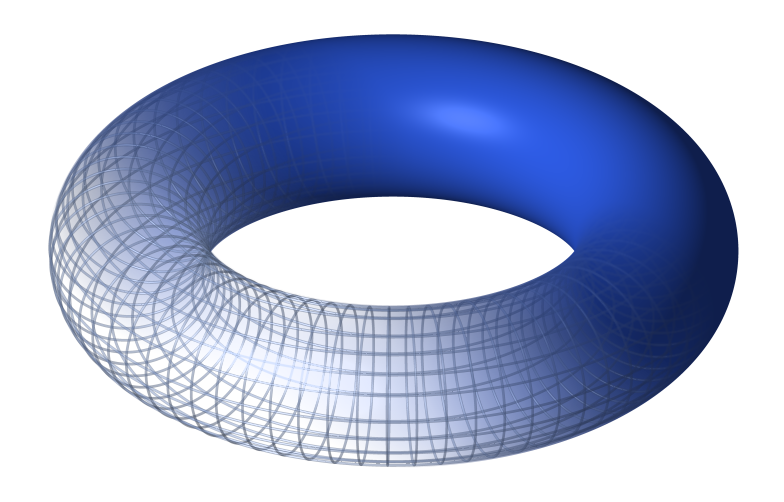
\includegraphics[width=0.8\textwidth]{figures/lez_16_Torus_low_quality.png}
    \caption{\scriptsize Toro in 3 dimensioni, ricordiamo che generalmente si parla di toro $n$ dimensionale.}
    \label{fig:figures-lez_16_Torus_low_quality-png}
\end{figure}
\noindent
\end{redbox}
\noindent
La dimostrazione è complicata, possiamo immaginarla visivamente pensando che il toro è l'unica varietà che, se considerata letteralmente pelosa, può essere pettinata. Una qualunque altra varietà, come una sfera ad esempio, presenterà delle stizze durante la pettinatura.
\begin{figure}[H]
    \centering
    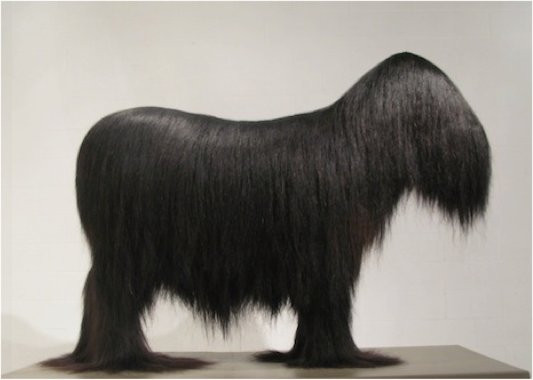
\includegraphics[width=0.4\textwidth]{figures/lez_15_toro_peloso.jpg}
    \caption{\scriptsize Un toro perfettamente pettinato}
    \label{fig:figures-lez_15_toro_peloso-jpg}
\end{figure}
\noindent
Formalmente se $\dot{\xi}$ è il campo di "velocità" che descrive il flusso di $H$ su $M$ il toro è l'unica varietà che permette di avere questo campo sempre tangente alla varietà stessa. 
\begin{figure}[H]
    \centering
    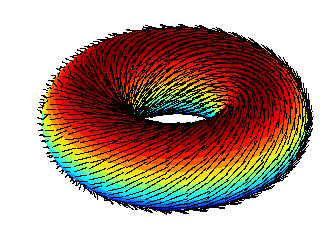
\includegraphics[width=0.2\textwidth]{figures/toroide_peloso.png}
    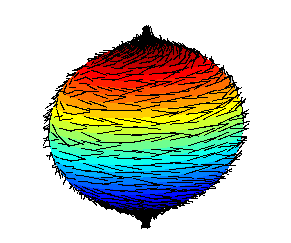
\includegraphics[width=0.2\textwidth]{figures/sfera_non_pettinabile}
    \caption{\scriptsize Un toroide pettinato ed una sfera non pettinabile (fonte: Wikipedia.)}
    \label{fig:figures-sfera_non_pettinabile}
\end{figure}
Nel caso 2-dimensionale ad esempio si ha che
\begin{redbox}{}
    La coppia di variabili azione-angolo è ben definita, infatti il toro è il prodotto di $n$ oggetti periodici.
\end{redbox}
\noindent
Tornando alle $n$ dimensioni si ha che:
\[
    I_k = \frac{1}{2\pi}\oint _{c_k} \sum_{i=1}^{n} p_idq_i
.\] 
Dove le $c_k $ sono traiettorie circuitate attorno al toro.\\
\begin{exmp}[Osillatore armonico bidimensionale.]
   \[
       H = \frac{1}{2}p_1^2+\frac{1}{2}p_2^2 + \frac{\omega_1^2}{2}q_1^2 + \frac{\omega_2^2}{2}q_2^2
   .\]  
   l'Hamiltoniana è separabile, quindi possiamo procedere definendo $\alpha_1$ e $\alpha_2$ come:
   \[
       \alpha_1 = \frac{1}{2}p_1^2+ \frac{\omega_1^2}{2}q_1^2 \qquad \alpha_2 = \frac{1}{2}p_2^2+ \frac{\omega_2^2}{2}q_2^2
   .\] 
   Abbiamo anche una coppia di azioni $I_{1,2}$:
   \[
       I_1 = \frac{1}{2\pi}\oint p_1dq_1 \qquad I_2 = \frac{1}{2\pi}\oint p_2dq_2 
   .\] 
   Mettendo tutto insieme nella Hamiltoniana trasformata finale si ottiene:
   \[
       H'(I_1,I_2) = \omega_1I_1+\omega_2I_2
   .\] 
\end{exmp}
\noindent
\subsection{Scrittura compatta del moto sul Toro}%
\label{sub:Scrittura compatta del moto sul Toro}
Il moto sul toro ha una struttura generale, possiamo riesprimerlo usando la periodicità nelle variabili azione-angolo.\\
Il nostro obiettivo finale è esprimere il moto della coordinata spaziale $q_i$ in funzione del tempo ($q_i(t)$). Nel sistema azione-angolo abbiamo che:
\[
    q_i(t) = q_i(\vect{I}, \vect{\theta}) 
.\] 
Possiamo allora cercare la decomposizione di Fourier di questa variabile nello spazio delle $I, \theta$ (essendo il moto periodico). \\
I pesi della trasformata sono:
\[
    \mathcal{A}_{\vect{k}}^{(i)}(\vect{I}) = \int_{0}^{2\pi} \theta_1 \ldots \int_{0}^{2\pi} \theta_n q_i(\vect{I}, \vect{\theta})e^{i(k_1\theta_1+ \ldots + k_n\theta_n) }   
.\] 
In cui $i$ è l'indice associato alla coordinata i-esima, $k$ è il pedice associato al $\theta$. \\
La decomposizione spettrale invece si esprime come:
\[\begin{aligned}
    q_i(t) = & \sum_{k_1=-\infty}^{\infty} \ldots\sum_{k_n = -\infty}^{\infty} \mathcal{A}_{k_1\ldots k_n}^{(i)} e^{i(k_1\theta_1+\ldots+k_n\theta_n)} =\\
	     & = \sum_{\vect{k}}^{} \mathcal{A}_{\vect{k}}^{(i)}e^{i(\vect{k}\vect{\omega} t + \vect{k}\vect{\delta}) }
.\end{aligned}\]
A questo punto la differenza tra il caso unidimensionale può esser vista in quest'ultima espressione: se gli $\omega_i$ stanno tra loro in rapporti razionali allora il moto sarà periodico chiuso, viceversa le orbite non si chiudono (nello spazio dei $q_i$).\\
In particolare per avere delle orbite chiuse servono $n-1$ relazioni del tipo:
\[
    \sum_{i=1}^{n} k_i\omega_i = 0
.\] 
\clearpage
